% Created 2017-12-03 Sun 15:42
\documentclass[11pt]{article}
\usepackage[utf8]{inputenc}
\usepackage[T1]{fontenc}
\usepackage{fixltx2e}
\usepackage{graphicx}
\usepackage{longtable}
\usepackage{float}
\usepackage{wrapfig}
\usepackage{rotating}
\usepackage[normalem]{ulem}
\usepackage{amsmath}
\usepackage{textcomp}
\usepackage{marvosym}
\usepackage{wasysym}
\usepackage{amssymb}
\usepackage{hyperref}
\tolerance=1000
\usepackage{xeCJK}
\setCJKmainfont{宋体}
\hypersetup{colorlinks=true,linkcolor=red}
\usepackage{minted}
\usepackage{geometry}
\geometry{left=2.0cm,right=2.0cm,top=2.5cm,bottom=2.5cm}
\setmainfont{Times New Roman}
\setsansfont{Arial}
\setmonofont{Courier New}
\usepackage{indentfirst}
\setlength{\parindent}{2em}
\author{MiracleEEEE}
\date{\today}
\title{Notes}
\hypersetup{
  pdfkeywords={},
  pdfsubject={},
  pdfcreator={Emacs 25.3.1 (Org mode 8.2.10)}}
\begin{document}

\maketitle
\tableofcontents


\section{基础算法}
\label{sec-1}

\subsection{位运算}
\label{sec-1-1}

\subsubsection{位运算的性质}
\label{sec-1-1-1}

$$x+y=x \& y + x | y$$ 

\subsubsection{输出整数的二进制表示}
\label{sec-1-1-2}

\begin{minted}[]{c++}
for (int i = 0; i < 32; ++i) {
  cerr << (a < 0);
  a <<= 1;
}
\end{minted}

\subsubsection{基本操作}
\label{sec-1-1-3}

\begin{center}
\begin{tabular}{ll}
操作 & 实现\\
\hline
去掉最后一位 & x >> 1\\
在最后加一个0 & x << 1\\
在最后加一个1 & (x << 1) or 1\\
把最后一位变成1 & x or 1\\
把最后一位变成0 & (x or 1) - 1\\
在最后一位取反 & x xor 1\\
右数第k位取反 & x xor (1 << k)\\
取末k位 & x and ((1 << k + 1) - 1)\\
末k位取反 & x xor ((1 << k + 1) - 1)\\
把右边连续的1变成0 & x and (x + 1)\\
把右起第一个0变成1 & x or (x + 1)\\
把右边连续的0变成1 & x or (x - 1)\\
取右边连续的1 & (x xor (x + 1)) >> 1\\
去掉右起第一个1的左边(lowbit) & x \& -x\\
\end{tabular}
\end{center}

\section{动态规划}
\label{sec-2}

\subsection{概述}
\label{sec-2-1}

动态规划是对状态空间进行分阶段、有顺序、无重复、决策性的遍历求解。

类比有向无环图的拓扑遍历。

三要素:阶段、状态、决策。

三前提:子问题重叠性、无后效性、最优子结构性质。

\subsubsection{动态规划的优化}
\label{sec-2-1-1}

当状态定义的过于严格时会造成转移的困难。这时候就需要在保证符合题意的情况下放宽一些限制,注意题目中的“或”,“至少”等关键词,往往可以从这些地方入手。或者观察状态转移方程,看看状态有没有什么可以化简的地方。如果数据范围很小,可以想想状态压缩。

\begin{enumerate}
\item 状态压缩
\label{sec-2-1-1-1}

当数据范围很小的时候可以想到的优化方法,可用位运算加速。
状态压缩后其实能从状态中得到很多信息,千万不要忽视这些信息。

\begin{enumerate}
\item 枚举子集
\label{sec-2-1-1-1-1}

设当前集合为 $S$ ,$S$ 的所有子集 $T$ 可以用 $T=(T-1) and S$ 得到,$T$ 的初值为 $S$ 。这样枚举 $S$ 集合,$S$ 集合的二进制表示的顺序为从大到小。如果想要保证按照二进制表示的大小从小到大枚举,可以令 $K=TxorS$ ,这样在,枚举 $T$ 的过程中 $K$ 的大小是递增的。 

\item 图形填充方案计数
\label{sec-2-1-1-1-2}


有些题目会给一张网格图和一些特殊的图形,求用这些图形填充这张网格图的方案数,特殊的地方在于,网格图的行数或者列数一般会很小。我们可以考虑对小的那一维状态压缩,一般的状态形如: $f[i][s]$ 表示第 $i$ 行状态为 $s$ 的方案数,可以视图形的特殊性考虑要不要附加上一行的状态。
\end{enumerate}
\end{enumerate}
\subsection{背包DP}
\label{sec-2-2}
\subsubsection{01背包}
\label{sec-2-2-1}

有 $N$ 件物品和一个容量为 $V$ 的背包。第 $i$ 件物品的体积是 $c[i]$ ,价值是 $w[i]$ 。求解将哪些物品装入背包可使价值总和最大。

每种物品仅有一件,可以选择放或不放。

用子问题定义状态:即 $f[i][v]$ 表示前 $i$ 件物品恰放入一个容量为 $v$ 的背包可以获得的最大价值。则其状态转移方程便是:
$$
f[i][v]=max\{f[i-1][v],f[i-1][v-c[i]]+w[i]\}
$$

可以使用滚动数组优化,优化之后的时间复杂度为 $O(VN)$ ,空间复杂度为 $O(V)$ 。

\begin{minted}[]{c++}
for (int i = 0; i < n; ++i) {
  for (int j = v; j > c[i]; --j) {
    f[j] = max(f[j], f[j - c[i]] + w[i]);
  }
}
\end{minted}

\subsubsection{完全背包}
\label{sec-2-2-2}

有 $N$ 件物品和一个容量为 $V$ 的背包。第 $i$ 件物品的体积是 $c[i]$ ,价值是 $w[i]$ 。每种物品无穷多件,求解将哪些物品放入背包可以使价值总和最大。

枚举选了 $k$ 件物品 $i$ 放入背包,类似01背包的状态定义,得到方程:

$$
f[i][v]=max\{f[i-1][v-k*c[i]]+k*w[i]|0 \leq k*c[i] \leq v\}
$$

时间复杂度为 $O(V*\sum_i V/c_i)$ 。

类似的使用滚动数组优化得到更简单的 $O(VN)$ 的状态转移方程。

\begin{minted}[]{c++}
for (int i = 0; i < n; ++i) {
  for (int j = c[i]; j <= v; ++j) {
    f[j] = max(f[j], f[j - c[i]] + w[i]);
  }
}
\end{minted}

\subsubsection{多重背包}
\label{sec-2-2-3}

有 $N$ 种物品和一个容量为 $V$ 的背包。第 $i$ 种物品最多有 $n[i]$ 件可用,每件体积是 $c[i]$ ,价值是 $w[i]$ 。求解将哪些物品装入背包可使这些物品的费用总和不超过背包容量,且价值总和最大。

基础的状态转移方程与完全背包类似:

$$
f[i][v]=max\{f[i-1][v-k*c[i]]+k*w[i]|0 \leq k \leq n[i]\}
$$

复杂度为  $O(V  \sum n[i])$ 。

\begin{enumerate}
\item 优化
\label{sec-2-2-3-1}

主要有两种优化:二进制拆分和单调队列。

\begin{enumerate}
\item 二进制拆分
\label{sec-2-2-3-1-1}


把 $n[i]$ 件物品i拆分成若干件物品,其体积和价值为原物品体积价值乘一个系数,然后用01背包算法解决。为了使我们解决的问题有意义,假设我们最优的选择方案选了 $k$ 件物品 $i$ ,考虑 $k$ 的二进制拆分, $k$ 一定能由几个 $2^m$ 的子物品拼成。一般的,任何一个10进制数都有其唯一存在的二进制表示,那么系数一般取 $1,2,4,8,16,...,2^{k-1},n[i]-2^{k}+1$ 。其中 $k$ 是满足 $n[i]-2^k+1>0$ 的最大整数。  
如果这样处理,那么一件物品就被拆成 $log(n[i])$ 件物品。对这些物品进行01背包即可。

\item 单调队列
\label{sec-2-2-3-1-2}


观察状态转移方程,难以发现一些优美的性质,考虑变形:  
设 $p=v/c_{i},r=v \mod c_i$ ,那么:

$$
f[i][p*c_i+r]=max\{f[i-1][(p-k)*c_i+r]+k*w[i]\}
$$

设 $m=p-k$ ,那么 $k=p-m$ :

$$
f[i][p*c_i+r]=max\{f[i-1][m*c_i+r]-m*w[i]+p*w[i]\}
$$

也就是

$$
f[i][p*c_i+r]=max\{f[i-1][m*c_i+r]-m*w[i]\}+p*w[i]
$$

现在这个式子就很有特点了,对于相同的 $r$ , $DP$ 数组的第二维关于 $m$ 相邻。  
那么,我们先枚举 $r$ ,然后枚举 $j$ ,用单调队列优化转移,先保证队头满足 $k=j-que[head].first \leq n[i]$ ,取队头更新: $f[i][j*c_i+r]=que[head].second+j*w[i]$ ,从队尾插入 $pair\{j,f[i-1][j*c_i+r]-j*w[i]\}$ 。总的时间复杂度 $O(V N)$ \footnote{代码中的v数组表示物品的体积,c数组表示物品的数量。}

\begin{minted}[]{c++}
memset(f, 0x3f, sizeof(f));
f[0] = 0;
for (int i = 0; i < n; ++i) {
  for (int r = 0; r < v[i]; ++r) {
    que.clear();
    for (int j = 0; j < k / v[i] + 1; ++j) {
      int s = j * v[i] + r;
      if (s > k) {
        break;
      }
      while (!que.empty() && j - que.front().first > c[i]) {
        que.pop_front();
      }
      int lst = f[s];
      if (!que.empty()) {
        f[s] = min(f[s], que.front().second + j);
      }
      while (!que.empty() && que.back().second >= lst - j) {
        que.pop_back();
      }
      que.push_back(mp(j, lst - j));
    }
  }
}
\end{minted}
\end{enumerate}
\end{enumerate}

\subsubsection{分组背包}
\label{sec-2-2-4}

给出 $N$ 组物品,其中第 \$i\$\$ 组有 $c[i]$ 个物品,第 $i$ 组的第 $j$ 个物品的体积为 $v[i][j]$ ,价值为 $w[i][j]$ ,有一个体积为 $V$ 的背包,要求选择若干个物品放入背包使得在每组至多选择一个物品并且物品总体积不超过 $V$ 的前提下有最大价值。

定义状态 $f[i][j]$ 表示在前 $i$ 组中选择容量为 $j$ 的物品的最大价值。状态转移方程:

$$
f[i][j]=max\{f[i-1][j],f[i-1][j-v[i][k]]+w[i][k]\}
$$

同理可以通过改变枚举策略压缩空间复杂度。

\begin{minted}[]{c++}
for (int i = 0; i < n; ++i) {
  for (int j = m; j >= 0; --j) {
    for (int k = 0; k < c[i]; ++k) {
      if (j - v[i][k] < 0) {
        continue;
      }
      f[j] = max(f[j], f[j - v[i][k]] + w[i][k]);
    }
  }
}
\end{minted}

\subsection{线性DP}
\label{sec-2-3}
\subsubsection{LIS}
\label{sec-2-3-1}

给定一个长度为 $N$ 的数列 $A$ ,求数值单调递增的子序列长度最长是多少。 $A$ 的任意子序列 $B$ 可以表示为 $B=\{A_{k_1},A_{k_2},...,A_{k_p}\}$ ,其中 \$ k$_{\text{1}}$ < k$_{\text{2}}$ < k$_{\text{3}}$ < $\cdots{}$ < k$_{\text{p}}$\$ 。

在实际题目中, $LIS$ 的模型可能会隐藏的很深。需要通过一些式子的变形来推导出能通过 $LIS$ 解决的模型。

定义: $f[i]$ 表示以 $A[i]$ 为结尾的最长上升子序列的长度,状态转移方程为:

$$
f[i]= \max_{0 \leq j < i,A[j] < A[i]} {f[j]+1}
$$

边界为 $f[0]=0$ ,目标为 $\max_{1 \leq i \leq N} {f[i]}$ 。

朴素实现的时间复杂度为 $O(n^2)$ 。

\begin{enumerate}
\item 优化
\label{sec-2-3-1-1}

相比于上面显然的状态设计,有另外一种巧妙的求 $LIS$ 的 $O(nlogn)$ 的递推算法。
令 $mn[i]$ 表示长度为 $i$ 的 $LIS$ 的最后一位最小是多少。贪心的想,较小的最后一位相比于较大的更优。而且, $mn$ 数组关于 $i$ 单调递增。于是有一个确定性的算法流程:初始化 $mn[i]=inf(1 \leq i \leq n),mn[0]=-inf$ 。对于第 $i$ 个数,我们找到当前最大的合法的 $len$ 满足 $mn[len] \leq A[i]$ ,并令 $mn[len+1]=min(mn[len+1],A[i])$ 。最后合法的 $mn[i] \neq inf$ 里最大的 $i$ 就是答案。寻找 $len$ 的过程可以二分实现,总时间复杂度 $O(nlogn)$ 。

\item 变形
\label{sec-2-3-1-2}

把一个序列 $A$ 变成非严格单调递增的(即单调不下降的),定义 $L$ 为 $A$ 的最长不下降子序列的长度,至少需要修改 $|A|-|{L}|$ 个数。
把一个序列 $A$ 变成单调严格递增,构造序列 $B=\{A[i]-i\}$ ,至少需要修改 $|A|-|{LIS_B}|$ 个数。
若非严格单调递增,那么对于一个不需要修改的 $A$ 的子序列 $C$ , $C$  需要满足 \$ C$_{\text{k}_{\text{1}}}$ < C$_{\text{k}_{\text{2}}}$ < C$_{\text{k}_{\text{3}}}$ < $\cdots{}$ < C$_{\text{k}_{\text{p}}}$\$ 。需要这样的子序列最长,减去 $|LIS|$ 即最小。如果是严格单调递增,对于任意两个不需要修改的数 \$A[i],A[j] (i < j) \$ ,需要满足 $A[j]-A[i] \geq j-i$ 。变形得到 $A[j]-j \geq A[i]-i$ 。转化为序列 $B$ 后得到与变形1类似的问题。
\end{enumerate}
\subsubsection{LCS}
\label{sec-2-3-2}

给定两个长度分别为 $N$ 和 $M$ 的字符串 $A$ 和 $B$ ,求既是 $A$ 的子序列,又是 $B$ 的子序列的字符串长度最长是多少。

令 $f[i][j]$ 表示前缀子串 $A[0 \sim i]$ , $B[0 \sim j]$ 的LCS的长度。状态转移方程:

$$ 
f[i][j]=max\left\{\begin{aligned}
&f[i-1][j]\\
&f[i][j-1]\\
&f[i-1][j-1]+1 (A[i]=A[j])
\end{aligned}\right. 
$$

边界: $f[i][0]=f[0][j]=0$ ,答案: $f[N-1][M-1]$ 
\subsubsection{数字三角形}
\label{sec-2-3-3}

给定一个共有 $N$ 行的三角矩阵 $A$ ,其中第 $i$ 行有 $j$ 列。从左上角出发,每次可以向下一步或者向右下方一步,并获得目标位置的价值,最终到达底部,求最大价值和。

令 $f[i][j]$ 表示从左上角走到位置 $(i,j)$ 的最大价值,状态转移方程:

$$
f[i][j]=A[i][j]+max\left\{\begin{aligned}
&f[i-1][j]\\
&f[i-1][j-1] (j>1)
\end{aligned}\right.
$$

边界 $f[0][0]=A[0][0]$ ,答案为 $\max_{0 \leq i \leq N-1} f[N-1][i]$ 。

\subsection{期望DP}
\label{sec-2-4}

期望和概率一般是互通的。

计算期望一般有两种方法:

\begin{itemize}
\item 根据期望的线性性质直接计算
\item 计算每一个随机变量的概率然后根据期望公式计算
\end{itemize}

一般情况下,终态确定时倒推,初态确定时正推。
\subsection{树形DP}
\label{sec-2-5}

\begin{enumerate}
\item 树形背包
\label{sec-2-5-0-1}

一般的状态转移方程形如:

$$
f[u][j] = max(f[u][j], f[v][k] + f[u][j - k])
$$

\item 树上支配问题
\label{sec-2-5-0-2}

一般可以根据题意列出一个直观的状态转移方程。然后可以视转移难度调整状态的设计,合适的状态设计很重要。
\end{enumerate}
\section{数学}
\label{sec-3}
\subsection{线性代数}
\label{sec-3-1}
\subsubsection{矩阵}
\label{sec-3-1-1}

\begin{enumerate}
\item 矩阵的图论意义
\label{sec-3-1-1-1}

定义 $A$ 为图 $G$ 的邻接矩阵,对于矩阵 $A^k$ , $a_{ij}$ 表示从点 $i$ 到点 $j$ 经过 $k$ 条边的路径条数。
\end{enumerate}
\subsubsection{线性基}
\label{sec-3-1-2}

\begin{enumerate}
\item 定义
\label{sec-3-1-2-1}

设数集 $T$ 的值域范围为 $[1,2^n-1]$ , $T$ 的线性基是是 $T$ 的一个生成子集 $A=\{a_0,a_1,a_2,\cdots,a_{n-1}\}$ 。 $A$ 中的元素互相 $xor$ 生成的集合,等价于原数集 $T$ 的元素相互异或形成的异或集合。

\item 性质
\label{sec-3-1-2-2}

\begin{enumerate}
\item 线性基的异或集合中不存在 $0$ 。
\item 线性基的异或集合中每一个元素的异或方案唯一。
\item 线性基二进制最高位互不相同。
\item 如果线性基是满的,那么它的异或集合为 $[1,2^n-1]$ 。
\item 线性基中的元素相互异或,异或集合不变。
\end{enumerate}

\item 操作
\label{sec-3-1-2-3}

\begin{enumerate}
\item 插入
\label{sec-3-1-2-3-1}

如果向线性基中插入数 $x$ ,那么从高到低扫描它为 $1$ 的二进制位。

扫描到第 $i$ 位时,如果 $a_i$ 不存在,就令 $a_i=x$ ,否则 $x=x \oplus a_i$ 。

$x$ 的结局是,要么被扔进线性基,要么经过一系列操作之后变成了 $0$ 。

\begin{minted}[]{c++}
for (int j = 50; j >= 0; --j) {
  if (x & (1ll << j)) {
    if (a[j]) {
      x ^= a[j];
    } else {
      a[j] = x;
      break;
    }
  }
}
\end{minted}

\item 合并
\label{sec-3-1-2-3-2}

将一个线性基中的元素插入到另一个即可。

\item 查询
\label{sec-3-1-2-3-3}

如果查询 $x$ 是否存在于 $A$ 的异或集合中,从高到底扫描它为 $1$ 的二进制位,扫描到第 $i$ 位的时候令 $x=x \oplus a_i$ 。如果中途 $x$ 变成了 $0$ ,那么说明存在,反之不存在。

\item 最大值
\label{sec-3-1-2-3-4}

从高到低位扫描线性基,如果异或后可以使答案变大,就异或到答案里去。

\item 最小值
\label{sec-3-1-2-3-5}

最小值即最低位上的线性基。

\item k小值
\label{sec-3-1-2-3-6}

首先将线性基改为每一位相互独立:对于 $i < j$ ,如果 $a_j$ 的第 $i$ 位为 $0$ ,那么就让 $a_j=a_j \oplus a_i$ ,同时删除等于 $0$ 的 $a_i$ 。查询的时候将 $k$ 二进制拆分,对于 $k$ 为 $1$ 的位,异或上对应的线性基。

\begin{minted}[]{c++}
inline void init() {
  for (int i = 0; i <= 50; ++i) {
    for (int j = i - 1; j >= 0; --j) {
      if (a[i] & (1ll << j)) {
        a[i] ^= a[j];
      }
    }
  }
  for (int i = 0; i <= 50; ++i) {
    if (a[i]) {
      b[cnt++] = a[i];
    }
  }
}

inline void query(int k) {
  int ret = 0;
  if (k >= (1ll << cnt)) {
    return -1;
  }
  for (int i = 50; i >= 0; --i) {
    if (k & (1ll << i)) {
      ret ^= a[i];
    }
  }
  return ret;
}
\end{minted}
\end{enumerate}
\end{enumerate}
\subsection{计算几何}
\label{sec-3-2}
\subsubsection{向量}
\label{sec-3-2-1}

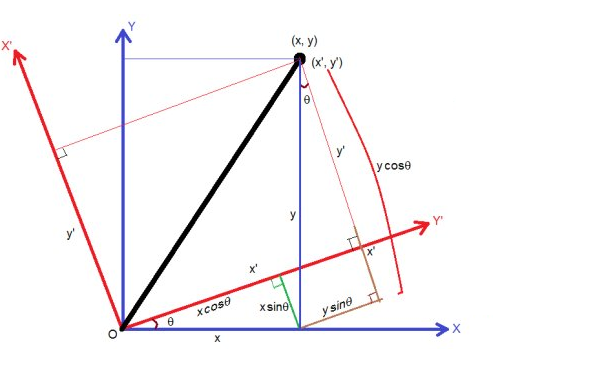
\includegraphics[width=.9\linewidth]{./Source/Picture/vector.png}

易得向量 $(x,y)$ 在顺时针旋转 $\theta$ 角后得到向量 $(x',y')$ 。其中

$$ \begin{aligned}
x'=xcos \theta+ysin\theta \\
y'=ycos \theta-xsin\theta
\end{aligned} $$

\subsubsection{曼哈顿距离}
\label{sec-3-2-2}
\begin{enumerate}
\item 转切比雪夫距离
\label{sec-3-2-2-1}

对于两个点 $A(x1,y1)$ , $B(x2,y2)$ 的曼哈顿距离等于 $|x_1-x_2|+|y_1-y_2|$ 。  

这个形式的式子往往不是很好处理,考虑转化:

拆绝对值:

$$ \begin{aligned}
x_1-x_2+y_1-y_2 \\
x_1-x_2+y_2-y_1 \\
x_2-x_1+y_1-y_2 \\
x_2-x_1+y_2-y_1
\end{aligned} $$

最后的答案就是四个式子中的最大值,那么等价于:

$$
max\{|(x_1+y_1)-(x_2+y_2)|,|(x_1-y_1)-(x_2-y_2)|\}
$$

设:

$$ \begin{aligned}
x_1'=x_1+y_1 \\
y_1'=x_1-y_1 \\
x_2'=x_2+y_2 \\
y_2'=x_2-y_2 \\
\end{aligned} $$


那么答案等于

$$
max\{|x_1'-x_2'|,|y_1'-y_2'|\}
$$
\end{enumerate}

\subsection{数论}
\label{sec-3-3}
\subsubsection{Lucas定理}
\label{sec-3-3-1}

$${\binom {m}{n}}\equiv \prod _{i=0}^{k}{\binom {m_{i}}{n_{i}}}{\pmod {p}}$$

其中
$$ \begin{aligned}
m = \sum_{i=0}^k m_i \cdot p^i\\
n=\sum_{i=0}^k n_i \cdot p^i\\
\end{aligned} $$

也可以表示成:

$$
\binom{m}{n} \equiv \binom{m \bmod p}{n \bmod p} \cdot \binom{\lfloor\frac{m}{p} \rfloor}{\lfloor \frac{n}{p} \rfloor} \pmod p
$$


\begin{enumerate}
\item 证明
\label{sec-3-3-1-1}

基于生成函数的证明:

如果 $p$ 为质数, $1\leq n \leq p-1$ ,那么

$$
\binom{p}{n} = \frac{p \cdot (p - 1) \cdots (p - n + 1)}{n \cdot (n - 1) \cdots 1}
$$

可得 $p$  是 $\binom{p}{n}$ 的一个因子。从生成函数的角度来说,这意味着

$$ \begin{aligned}
(1 + X)^p &= \sum_{i=0}^p \binom{p}{i}\cdot X^i\\
&\equiv 1+X^p \pmod p
\end{aligned} $$

类似的,对于每个非负整数 $i$ ,有

$$
(1+X)^{p^i} \equiv 1 + X^{p^i} \pmod p
$$

令非负整数 $m=\sum_{i=0}^k m_i p^i$ , 那么

$$ \begin{aligned}
\sum_{n=0}^m \binom{m}{n}X^n &= (1 + X)^m \\
&=\prod_ {i=0}^k \Big ((1+X)^{p^i} \Big) ^{m_i}\\
&\equiv \prod_{i=0}^k(1+X^{p^i})^{m_i}\\
&=\prod_{i=0}^k\bigg ( \sum_{n_i=0}^{m_i} \binom{m_i}{n_i}X^{n_i p^i} \bigg)\\
&=\prod_{i=0}^k \bigg (\sum_{n_i=0}^{p-1} \binom{m_i}{n_i}X^{n_ip^i} \bigg)\\
&=\sum_{n=0}^m \bigg(\prod_{i=0}^k \binom{m_i}{n_i} \bigg) X^n \pmod p
\end{aligned} $$

得证,最后一步化简可由上一步展开观察得到。其中, $m_i$ , $n_i$ 分别是 $m$ 和 $n$ 在 $p$ 进制下的第 $i$ 位。

\item 结论
\label{sec-3-3-1-2}

组合数 $\binom{m}{n}$ 能被质数 $p$ 整除当且仅当存在至少一个 $i$ 使得在 $n$ 和 $m$ 在 $p$ 进制下有 $n_i > m_i$ 成立。
\end{enumerate}
% Emacs 25.3.1 (Org mode 8.2.10)
\end{document}
